%
%\documentclass[preprint,aps,superscriptaddress,showpacs,amsmath]{revtex4}
\documentclass[superscriptaddress,12pt,amsmath]{revtex4-2}		
\usepackage{graphicx}
\usepackage{color}
\usepackage{hyperref}% add hypertext capabilities

\graphicspath{{figures_manuscript/}}
\usepackage{verbatim}
\usepackage[normalem]{ulem}  
%\usepackage[babel}  
\newcommand{\mcC}{\mathcal{C}} 
\newcommand{\mcH}{\mathcal{H}} 	%Hamiltonian
\providecommand{\abs}[1]{\left\lvert#1\right\rvert}
\providecommand{\norm}[1]{\lVert #1 \rVert}
\providecommand{\vxp}[1]{\langle #1 \rangle}
\providecommand{\bra}[1]{\langle #1 \rvert}
\providecommand{\ket}[1]{\lvert #1 \rangle}
\providecommand{\bbra}[1]{\langle #1 \rvert\rvert}
\providecommand{\kket}[1]{\lvert\lvert #1 \rangle}
\providecommand{\kkket}[1]{\lvert #1 \rangle\rangle}
\providecommand{\braket}[2]{\langle #1 \rvert #2 \rangle}
%\providecommand{\vxp3}[3]{\langle #1 |#2| #3 \rangle}
\providecommand{\tr}[1]{\text{tr}\left[ #1 \right]}
\newcommand{\ketbra}[2]{\left| {#1} \right\rangle\left\langle {#2}\right|}

\begin{document} 

\title{Resonancia Fluorescente Intermitente}  
 
\author{H\'ector M. Castro-Beltr\'an} 
\email{hcastro@uaem.mx}
\affiliation{Centro de Investigaci\'on en Ingenier\'ia y Ciencias Aplicadas, 
Instituto de Investigaci\'on en Ciencias B\'asicas y Aplicadas, \\ 
Universidad Aut\'onoma del Estado de Morelos, 
Avenida Universidad 1001, 62209 Cuernavaca, Morelos, M\'exico}
\author{Kevin Mart\'inez Franco} 
\email{hcastro@uaem.mx}
\affiliation{Centro de Investigaci\'on en Ingenier\'ia y Ciencias Aplicadas, 
Instituto de Investigaci\'on en Ciencias B\'asicas y Aplicadas, \\ 
Universidad Aut\'onoma del Estado de Morelos, 
Avenida Universidad 1001, 62209 Cuernavaca, Morelos, M\'exico}

%\draft 
\date{\today}
\begin{abstract}
Estudiamos te\'oricamente el parpadeo de la fluorescencia de un \'atomo 
individual excitado continuamente por un l\'aser e interrumpida aleatoriamente 
por decaimiento a un estado metaestable. La interrupci\'on y reinicio de la 
fluorescencia son interpretados como saltos cu\'anticos. Utilizamos 
ecuaciones estoc\'asticas discontinuas y difusivas para simular 
fotoconteo y detecci\'on heterodina de la fluorescencia; la segunda de 
ellas nos lleva a obtener el espectro, cuya caracter\'istica especial es un 
pico muy angosto de anchura cercana a la vida media del estado metaestable. 
\end{abstract}

%\pacs{42.50.Lc, 42.50.Md, 32.80.-t}
%\keywords{resonance fluorescence, electron shelving, blinking, quantum 
%jumps, time-dependent spectra.}
\maketitle

%%%%%%%%%%%%%%%%%%%%%%%%%%%%%% new section
\section{Introducci\'on}

 %%%%%%%%%%%%%%
 %\subsection{Saltos Cu\'anticos de Bohr}
En 1913, Neils Bohr postul\'o que las energ\'ias posibles del electr\'on en 
un \'atomo de hidr\'ogeno est\'an cuantizadas, es decir, discretizadas, y 
que los electrones se mueven en \'orbitas circulares estables \cite{Bohr13}. 
El electr\'on puede pasar de una \'orbita de energ\'ia $E_n$ a otra de 
energ\'ia $E_m$, $n,m =1,2,3,\ldots$, emitiendo o absorbiendo un cuanto 
de luz o fot\'on de energ\'ia 
%
\begin{eqnarray} 		%\label{eq:phEnergy}
\hbar \omega_{nm} = E_R \left( \frac{1}{n^2} -  \frac{1}{m^2} \right) \,, 
	\qquad 
E_R = \frac{m_e e^4}{8 \epsilon_0^2 h^2 } = 13.60 \,\mathrm{eV} 	\,,
\end{eqnarray}
%%
donde $E_R$ es la energía de Rydberg. Este salto es discontinuo si lo 
vemos desde el punto de vista del átomo, porque dijimos que las órbitas 
son estables. Sin embargo, también sabemos que la luz tiene aspecto 
ondulatorio, por lo que el fotón se vería como un paquete de onda con 
extensión finita. 

En 1975, a fin de estudiar espectroscopía de transiciones débiles, Hans 
Dehmelt \cite{Dehmelt75} propuso saltos donde la fluorescencia de una 
transici\'on fuerte, en la que se emiten muchos fotones al ser iluminada 
por un l\'aser, es interrumpida por la transición del electrón a un estado 
de larga vida media o mestaestable, en un efecto llamado \textit{electron 
shelving} \cite{NaSD86}. El átomo regresa eventualmente al estado base 
emitiendo un fotón. Al continuar la excitaci\'on por el l\'aser contin\'ua la 
fluorescencia. En este proceso tenemos entonces dos saltos: el primero 
consiste en la interrupción abrupta de la fluorescencia de la transición 
fuerte, y el segundo en el retorno a la fluorescencia. 

El proceso de emisi\'on espont\'anea de fotones mientras el \'atomo es 
iluminado se denomina resonancia fluorescente. En el caso descrito 
arriba se tiene que \'esta es intermitente, con per\'iodos brillantes, con la 
emisi\'on de muchos fotones, y oscuros, sin luz. Muchos experimentos 
han demostrado el efecto de intermitencia, obteniendo la distribuci\'on 
de la duraci\'on de los per\'iodos brillantes y oscuros y otras propiedades 
\cite{NaSD86,SNBT86,BHIW86,PlKn98,BuTa00}. 

La modulaci\'on estoc\'astica de la fluorescencia tambi\'en tiene su efecto 
en el espectro o distribuci\'on en frecuencias, produciendo un pico muy 
angosto, varios \'ordenes menor que el de emisi\'on espont\'anea, 
producido en transiciones muy d\'ebiles, tales como cuadrupolar y 
octupolar el\'ectricas. El pico angosto es la evidencia espectral del 
decaimiento aleatorio hacia un estado metaestable que interrumpe la 
fluorescencia en la transici\'on fuertemente iluminado por un l\'aser  \cite{HePl95,GaKK95}. Este pico fue medido por B\"uhner y Tamm con 
un i\'on individual de $^{171} \mathrm{Yb}^+$ mediante detecci\'on 
heterodina \cite{BuTa00}. Posteriormente, Evers y Keitel \cite{EvKe02} 
demostraron que este pico angosto incoherente se forma a expensas de la 
parte coherente del espectro, y Castro-Beltr\'an \textit{et al} \cite{CaRG16} 
obtuvieron una soluci\'on anal\'itica muy precisa para los par\'ametros de inter\'es. 

En este trabajo realizamos un estudio te\'orico-computacional de la 
resonancia fluorescente intermitente (RFI) usando ecuaciones 
estoc\'asticas de Schr\"odinger (EES). Primero, usando EES discont\'inuas, 
simulamos la formaci\'on de los per\'iodos brillantes y oscuros y obtenemos 
distribuciones de probabilidad de ocurrencia de dichos eventos. 
Destacamos entre ellas, la de los intervalos entre dos ciclos de un per\'iodo 
oscuro seguido de uno brillante, que llamamos distribuci\'on de tiempos de 
retorno, que realza la din\'amica a tiempos largos. Despu\'es, con EES 
difusivas, obtenemos el espectro mediante la simulaci\'on del proceso de 
detecci\'on heterodina de la luz. Finalmente, de \cite{CaRG16}, obtenemos 
resultados complementarios usando el m\'etodo de ecuaci\'on maestra para 
el operador de densidad del \'atomo. 

%%%%%%%%%%%%%%%%%%%%%%%%%%%%%% new section
\section{Modelo}
El sistema, mostrado en la Figura \ref{fig:3LA}, consiste en un \'atomo 
o mol\'ecula individual con tres niveles de energ\'ia relevantes: un estado 
base $|g\rangle$ acoplado con un estado de mayor energ\'ia $|e\rangle$ 
mediante un l\'aser monocrom\'atico; esta interacci\'on est\'a descrita 
por la frecuencia de Rabi $\Omega$. De la teor\'ia de Einstein de la 
radiaci\'on sabemos que el \'atomo emite luz de manera estimulada en 
respuesta al l\'aser, en la misma direcci\'on y fase que \'este, y que 
tambi\'en emite luz de manera espont\'anea con un patr\'on dipolar. En 
los experimentos que estudiamos solo observamos la luz emitidad en 
direcci\'on perpendicular al l\'aser, por lo que solamente interesa la de
emisi\'on espont\'anea. 
%
\begin{figure}[b]
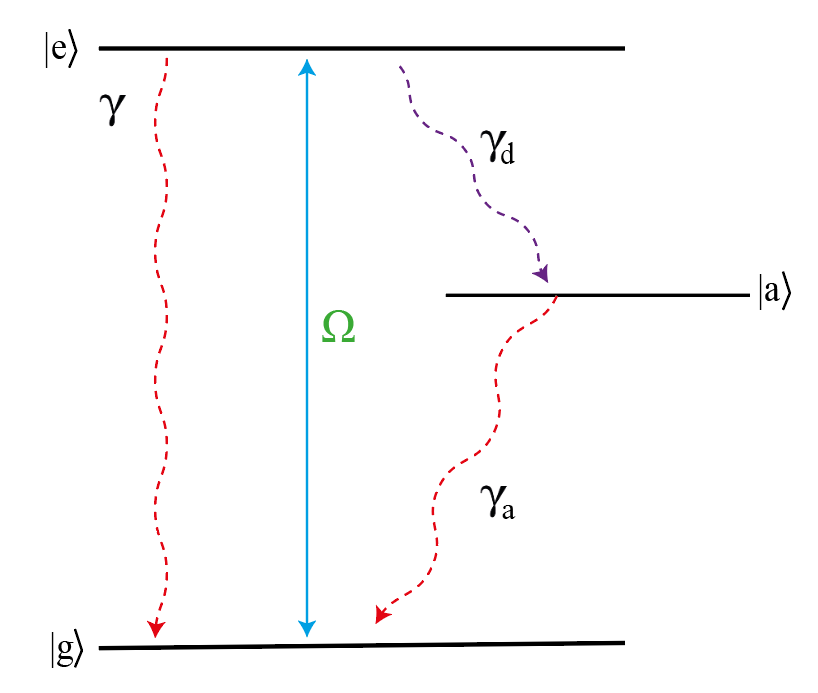
\includegraphics[width=11cm,height=6.0cm]{fig1_sistema.png}
\caption{\label{fig:3LA}  
Esquema de niveles de energ\'ia del \'atomo en fluorescencia resonante intermitente.  }
\end{figure}
%% 

La transici\'on $|g\rangle - |e\rangle$ es denominada dipolar fuerte, lo 
que significa que el \'atomo se acopla fuertemente al l\'aser y $|e\rangle$ 
decae r\'apidamente a $|g\rangle$, emitiendo fotones a raz\'on 
$\gamma \sim 10^8 \,\mathrm{Hz}$. Sin embargo, el estado $|e\rangle$ 
puede decaer tambi\'en a otro estado $|a\rangle$, una transici\'on dipolar 
m\'as d\'ebil con decaimiento $\gamma_d \sim 10^{5} \,\mathrm{Hz}$. 
Este estado decae finalmente al estado $|g\rangle$ pero, por reglas de 
selecci\'on de momento angular, la transici\'on $|a\rangle -|g\rangle$ es 
cuadrupolar, muy d\'ebil, decayendo a raz\'on 
$\gamma_a \sim 10^{3} \,\mathrm{Hz}$. Decimos, entonces, que 
$|a\rangle$ es un estado metaestable, cuya vida media 
$\tau_a =\gamma_a^{-1}$ es muy larga. Todo esto nos lleva a que la 
fluorescencia en la transici\'on fuerte, con la emisi\'on de muchos fotones 
(per\'iodo brillante), se ve interrumpida aleatoriamente, creando per\'iodos 
sin luz (per\'iodos oscuros). Esto es la resonancia fluorescente 
intermitente. La condici\'on para que ocurra es que 
$\Omega \sim \gamma \gg \gamma_d, \gamma_a$. 
 
Se han realizado experimentos de resonancia fluorescente  intermitente de 
un ion de Yterbio en una trampa de Paul \cite{BuTa00}. La Fig.~\ref{fig:3LA} 
muestra los niveles relevantes del proceso. La raz\'on de decaimiento total 
del estado $|e\rangle$ es $\gamma_+ \simeq 23$ MHz, con probabilidad 
99.95\% al estado $|g\rangle$ y 0.05\% al estado $|a\rangle$. Por ello 
utilizaremos los valores $\gamma_e \simeq \gamma =1$ y 
$\gamma_d =0.05$. La raz\'on $\gamma_a$ es en realidad un par\'ametro 
ajustable para acelerar un poco el decaimiento al estado  $|g\rangle$ en 
el que se usa un l\'aser ruidoso para acoplar $|a\rangle$ con un cuarto 
estado $|c\rangle$ que s\'i decae r\'apidamente a $|g\rangle$, pero a\'un 
cumpliendo la condici\'on $\gamma_a < \gamma_d \ll \gamma$ 
\cite{BuTa00}. Nos limitamos al valor $\gamma_a = 0.015 \gamma$.
 
%%%%%%%%%%%%%%%%%%%%%%%%%%%%%% new section
\section{Trayectorias Cu\'anticas Discont\'inuas: Fotoconteo y 
Simulaci\'on de Saltos}
Resolvemos la ecuaci\'on de Schr\"odinger 
$i \hbar \ket{\dot{\Psi}_c} = H_{\mathrm{eff}} \ket{\Psi}_c$, donde 
$H_{\mathrm{eff}}$ es un Hamiltoniano efectivo no hermitiano,  
%
\begin{eqnarray}
H_{\mathrm{eff}} = \hbar \Delta \sigma_{ee} 
	+ \hbar \frac{\Omega}{2}(\sigma_{eg}  +\sigma_{ge}) 
 	-i \hbar \frac{\gamma+\gamma_d}{2} \sigma_{ee} 
	 -i \hbar \frac{\gamma_a}{2} \sigma_{aa} \,, 
\end{eqnarray}
%%
cuyos dos \'ultimos t\'erminos indican decaimiento por emisi\'on de fotones, 
$\sigma_{jk} = |j\rangle \langle k|$ son operadores del \'atomo, $\Omega$ 
es el acoplamiento \'atomo-l\'aser,  $\Delta= \omega_{eg} -\omega_L$ es la 
desinton\'ia \'atomo-l\'aser, y $\hbar$ es la constante de Planck reducida 
($\hbar=h/2\pi$). 

Puesto que la evoluci\'on no es unitaria, la funci\'on de onda 
%
\begin{equation}
\ket{\bar{\Psi}_c (t)} = \bar{c}_g(t) \ket{g} +\bar{c}_e(t) \ket{e} 
	+\bar{c}_a(t) \ket{a} 
\end{equation}
%%
no est\'a normalizada, por lo que la debemos normalizar cada intervalo 
$\delta t$ (del orden de $1/100\gamma$), 
%
\begin{figure}[t]
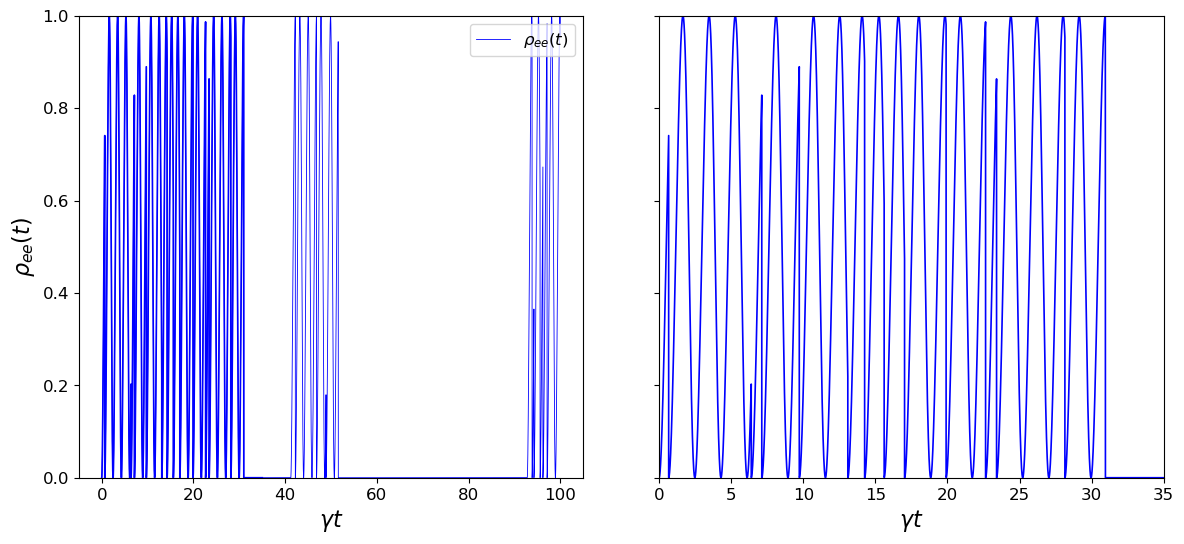
\includegraphics[width=15cm,height=6cm]{fig2_Trayectoria_saltos.png}
\caption{\label{fig:3LA-tray} Probabilidad de ocupaci\'on del estado 
excitado $|e\rangle$; $\Omega = 3.5 \gamma$, 
$\gamma_d = 0.05\gamma$, $\gamma_a = 0.015 \gamma$. 
(a) Segmento de una trayectoria estoc\'astica con per\'iodos brillantes 
y oscuros; (b) segmento que muestra detalle de las oscilaciones de 
Rabi interrumpidas por la emisi\'on de un fot\'on (l\'ineas verticales) 
y entrada a un per\'iodo oscuro. \textcolor{red}{Cambiar $\rho_{ee}(t)$ 
por $|c_e|^2$}.  }
\end{figure}
%% 
%
\begin{eqnarray}
\ket{\Psi_c} &=& \frac{ \ket{\bar{\Psi}_c} }
	{ \sqrt{ \braket{ \bar{\Psi}_c}{\bar{\Psi}_c}  }  } \,, \qquad 
\braket{ \bar{\Psi}_c}{\bar{\Psi}_c} = |\bar{c}_e|^2 +|\bar{c}_a|^2 
	+|\bar{c}_g|^2	\,.\qquad 
\end{eqnarray}
%%
La propagaci\'on se realiza hasta que ocurre la emisi\'on de un fot\'on, 
con el consecuente salto al estado inferior de la transici\'on, colapsando 
la funci\'on de onda. Por ejemplo, 
$\mathcal{C}_e = \sqrt{\gamma} \,\sigma_{ge}$ 
es el operador que indica la emisi\'on de un fot\'on en la transici\'on 
$\ket{e} - \ket{g}$, entonces  
%
\begin{equation}
\ket{\bar{\Psi}_c} \to \mathcal{C}_e \ket{\bar{\Psi}_c} 
	= \sqrt{\gamma} \,c_e \ket{g} \,. 
\end{equation}
%%
Aqu\'i tenemos tres operadores de salto: 
%
\begin{equation}
\mcC_e = \sqrt{\gamma} \,\sigma_{ge} \,, \qquad 
	\mcC_d = \sqrt{\gamma_d} \,\sigma_{ae} \,, \qquad 
	\mcC_a = \sqrt{\gamma_a} \,\sigma_{ga} \,. 
\end{equation}
%%

Como los saltos ocurren aleatoriamente calculamos la probabilidad 
de que ocurran,
%
\begin{eqnarray}
p_k(t) &=& \delta t \bra{\Psi_c (t)} \mcC_k^\dag \mcC_k \ket{\Psi_c (t)} 	\,, 
	\qquad k=e,d,a \,, 
\end{eqnarray}
%%
Para cada intervalo de tiempo $\delta t$ estas probabilidades deben ser 
comparadas con n\'umeros aleatorios $r_k \in (0,1)$. Si $p_k(t) > r_k$ 
entonces se produce la emisi\'on de un fot\'on; de lo contrario, la funci\'on 
de onda evoluciona de forma cont\'inua --- por supuesto, el algoritmo 
debe considerar que ocurre emisi\'on solamente en una transici\'on en el 
intervalo $\delta t$. La Fig.~\ref{fig:3LA-tray} muestra un fragmento de 
una larga historia de per\'iodos brillantes y oscuros. Tras cada salto 
tambi\'en hay que normalizar la funci\'on de onda, 
%
\begin{eqnarray}
|\Psi (t) \rangle = \frac{\mcC_k \ket{\bar{\Psi}_c (t)} }
	{ \bra{\bar{\Psi}_c (t)} \mcC_k^\dag \mcC_k \ket{\bar{\Psi}_c (t)} }  	\,, 
\end{eqnarray}
%%
y continuar la evoluci\'on. 

Tenemos entonces que $\ket{\Psi_c (t)}$ es la funci\'on de onda 
(normalizada) con una historia particular de saltos mediados por 
per\'iodos de evoluci\'on cont\'inua. Estas Trayectorias Cu\'anticas de 
saltos simulan experimentos de medici\'on por fotoconteo, en los que 
este algoritmo permite recoger datos sobre la estad\'istica de la emisi\'on 
de fotones, que veremos a continuaci\'on.

%%%%%%%%%%%%%%%%%%%%%%%%%%%%%% new section
\subsection{Estad\'istica de Per\'iodos Brillantes y Oscuros 
\label{ss:PeriodsStats}}
La informaci\'on que salta primero a la vista es la de la duraci\'on de los 
per\'iodos brillantes y oscuros. Se pueden calcular las duraciones 
promedio usando un modelo sencillo de tel\'egrafo aleatorio 
\cite{EvKe02,PeKn88,CaRG16}. Se parte de la ecuaci\'on para la 
probabilidad de ocupaci\'on (poblaci\'on) del estado metaestable $|a\rangle$,
$\dot{\rho}_{aa} = \gamma_d \rho_{ee} - \gamma_a \rho_{aa}$, donde 
$\rho_{ee}$ es la poblaci\'on del estado $|e\rangle$. Durante un per\'iodo 
brillante el estado $|a \rangle$ nunca esta ocupado, $\rho_{aa}(t) =0$. 
El per\'iodo brillante promedio $T_B$ se define como 
$T_B^{-1} = (\dot{\rho}_{aa})_{t \to \infty}$, donde el l\'imite significa un 
tiempo suficientemente largo para que la transici\'on del subsistema de 
dos niveles (A2N) $|g \rangle - |e \rangle$ alcance el estado estacionario, 
tal que  $\rho_{ee}(\infty) \to (\rho_{ee}^{st})_{A2N}$, obteniendo 
%
\begin{eqnarray}    \label{eq:AvBrightPeriod}
T_B = \frac{2\Omega^2 +\gamma^2 +4\Delta^2}
  	{\gamma_d \Omega^2} \,. 		
\end{eqnarray}
%%  
Similarmente, el per\'iodo oscuro promedio se define como  
$T_D^{-1} = (\dot{\rho}_{aa})_{t \to \infty}$ pero, durante un per\'iodo 
oscuro $\rho_{aa}(t) =1$ and $\rho_{ee}(t) = 0$, por lo que  
%
\begin{eqnarray}    \label{eq:AvDarkPeriod}
	T_D = \gamma_a^{-1} 	\,.
\end{eqnarray}
%% 

Los per\'iodos brillantes promedio dependen mucho de la frecuencia de 
Rabi $\Omega$, tal que $T_B >40/\gamma$, pero son del mismo orden 
que los de tiempos oscuros, $T_D =\gamma_a^{-1} \simeq 67/\gamma$,  
usando los par\'ametros $\Omega = 3.5 \gamma$, 
$\gamma_d = 0.05\gamma$, $\gamma_a = 0.015 \gamma$. 
Las duraciones de los per\'iodos brillantes y oscuros siguen una 
distribuci\'on de Poisson, 
%
\begin{figure}[t]
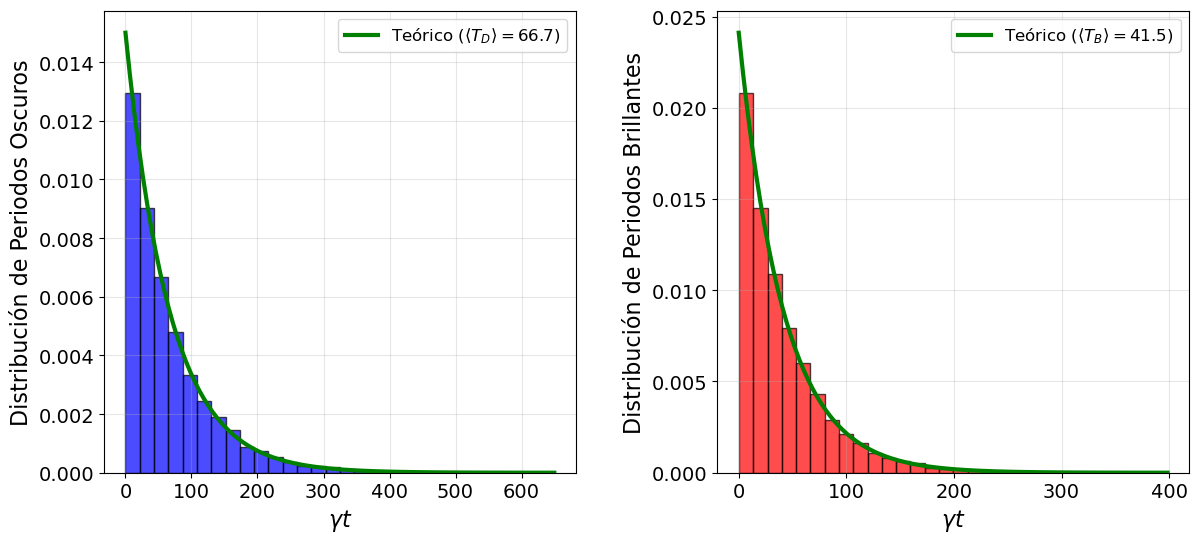
\includegraphics[width=15cm,height=6.0cm]{fig3_distribucion_periodos.png} 
\caption{\label{fig:Dist_periodos} Distribuciones de per\'iodos (a) oscuros 
y (b) brillantes, con $\Omega = 3.5 \gamma$, 
$\gamma_d = 0.05\gamma$, $\gamma_a = 0.015 \gamma$. 
Las l\'ineas verdes son de las Ecs.(\ref{eq:Dist_periodos}). }
\end{figure}
%% 
%
\begin{equation} 	\label{eq:Dist_periodos}
P_B = \frac{1}{T_B} e^{-t/T_B} \,, 	\qquad 
	P_D = \frac{1}{T_D} e^{-t/T_D} \,.
\end{equation}
%% 
La Fig.~\ref{fig:Dist_periodos} muestra las distribuci\'on de intervalos 
oscuros y brillantes. Se pueden apreciar algunos per\'iodos oscuros muy 
largos, mientras que los per\'iodos oscuros muy cortos podr\'ian no estar 
muy bien definidos porque pueden confundirse con intervalos 
inusualmente largos entre dos fotones dentro de un per\'iodo brillante, 
como se ve en la siguiente subsecci\'on.

%%%%%%%%%%%%%%%%%%%%%%%%%%%%%% new section
\subsection{Distribuci\'on de tiempos de espera}
%
\begin{figure}[b]
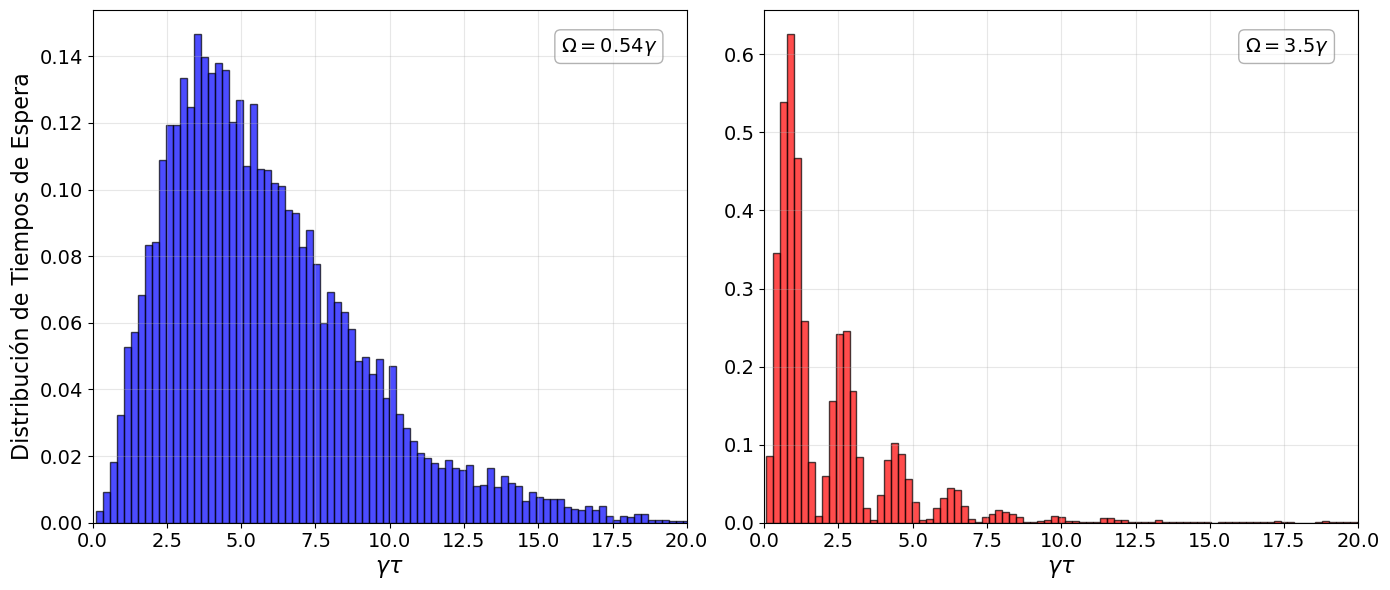
\includegraphics[width=15cm,height=6.0cm]{fig4_waiting_time_dist.png} 
\caption{\label{fig:3LA-wait} Distribuci\'on de tiempos de espera con 
$\gamma_d = 0.05\gamma$, $\gamma_a = 0.015 \gamma$ y  
excitaci\'on moderada, $\Omega=0.54 \gamma$ (izq.), y excitaci\'on 
fuerte, $\Omega=3.5 \gamma$ (der.). Los \'ultimos datos de las 
simulaciones, fuera de las gr\'aficas, son $\gamma \tau = 471$ y 
$\gamma \tau = 468$, respectivamente. }
\end{figure}
%% 
Esta distribuci\'on, tambi\'en llamada funci\'on de retardos, se refiere al 
intervalo entre la emisi\'on de dos fotones consecutivos de la transici\'on 
fuerte, $w_{eg}(\tau) = \gamma |c_e(\tau)|^2$. La duraci\'on promedio 
de estos intervalos o raz\'on de fotoemisi\'on es 
%
\begin{eqnarray} 	\label{eq:meantau}
 \bar{\tau} &=& \int_0^{\infty} \tau w_{eg}(\tau) d\tau  	\nonumber \\
	&=& \frac{1}{\gamma \rho_{ee}^{st} } 	
	= \frac{(2 +q)\Omega^2 +\gamma_+^2 +4 \Delta^2}
	{\gamma \Omega^2} 	\,,		
\end{eqnarray}
%% 
donde $\rho_{ee}^{st}$ es la probabilidad estacionaria de ocupar el 
estado $|e\rangle$ y $q=\gamma_d/\gamma_a$ \cite{CaRG16}. Por 
supuesto, puede ocurrir un per\'iodo oscuro entre estos dos fotones y 
mostrarse en intervalos muy largos, Fig.~\ref{fig:3LA-wait}, mucho 
mayores que $\Omega^{-1}$, que es el tiempo m\'as probable para la 
emisi\'on de un fot\'on después de haber estado en el estado base. 

Una aplicaci\'on de esta distribuci\'on es que puede usarse para calcular 
la probabilidad de la emisi\'on de un fot\'on en simulaciones de trayectorias 
de saltos. Esto supondr\'ia, sin embargo, duplicidad en los c\'alculos: 
obtener primero un gran ensamble de trayectorias y generar 
$w_{eg}(\tau)$ y luego obtener trayectorias individuales u otro ensamble. 

Un problema con esta distribuci\'on es que supone eficiencia de colecci\'on 
y detecci\'on de fotones unitaria, por lo que en la pr\'actica se utilizan las 
correlaciones foton-fot\'on, que no implican fotones consecutivos. No nos 
ocuparemos de ellas en este art\'iculo. 

%%%%%%%%%%%%%%%%%%%%%%%%%%%%%% new section
\subsection{Distribuci\'on de tiempos de retorno}
Los tiempos oscuros sugieren que se mida la distribuci\'on de tiempos en 
los que el \'atomo pasa un tiempo oscuro y uno brillante, $w_{aa} (\tau)$, 
iniciando en el estado metaestable. El tiempo promedio para dichos 
retornos es $T_D +T_B$, pero la larga cola de la distribuci\'on, mostrada 
en la Fig.~\ref{fig:w_aa}, evidencia claramente el efecto de los per\'iodos 
oscuros, no muy bien resueltos en $w_{eg}(\tau)$, que es claramente 
dominada por intervalos cortos. Tambi\'en se aprecia que 
$w_{aa}(\tau =0) \neq 0$, indicando que  un decaimiento de $|a\rangle$ 
a $|g\rangle$ a tiempos muy cortos es probable, aunque, de nuevo, puede 
confundirse en un per\'iodo brillante. Adem\'as, experimentalmente, implica 
que debe ocurrir un tiempo umbral que indique que termin\'o un per\'iodo 
brillante. La utilidad de $w_{aa} (\tau)$ radica entonces en la informaci\'on 
que proporciona a intervalos largos.  
%
\begin{figure}[b]
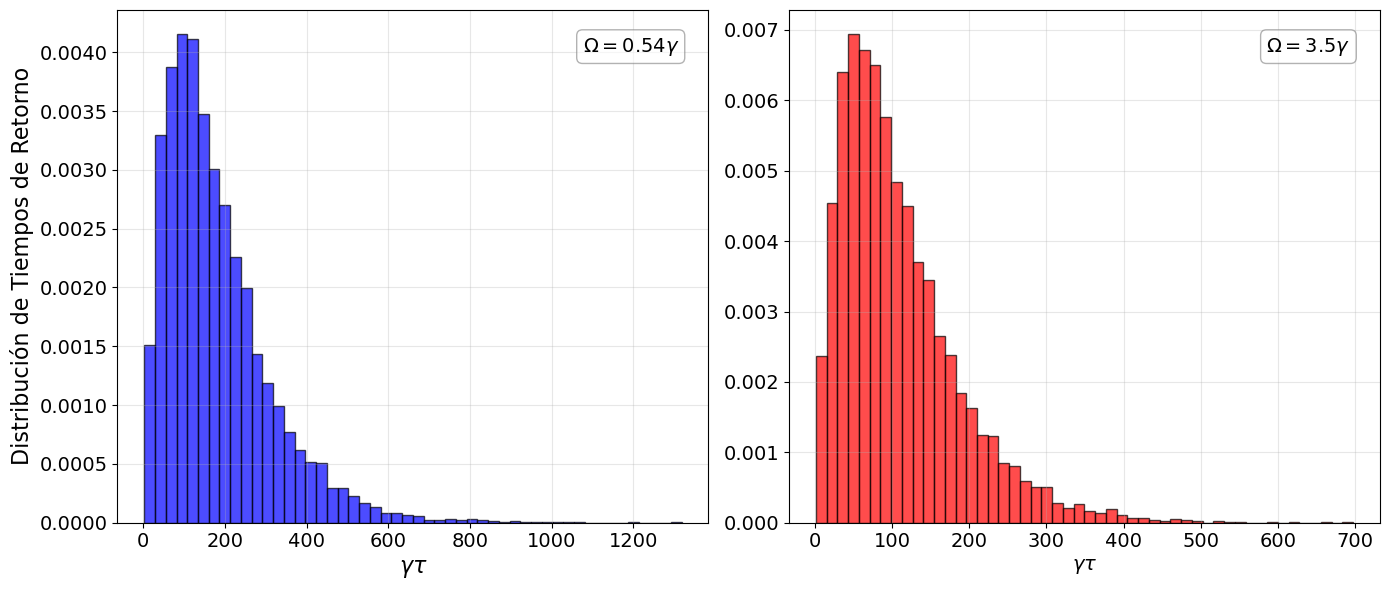
\includegraphics[width=15cm,height=6.0cm]{fig5_return_times.png} 
\caption{\label{fig:w_aa} Distribuci\'on de tiempos de retorno. 
$\Omega=0.54 \gamma$ (izquierda), $\Omega=3.5 \gamma$ (derecha) 
y $\gamma_d = 0.05\gamma$, $\gamma_a = 0.015 \gamma$.}
\end{figure}
%% 

%%%%%%%%%%%%%%%%%%%%%%%%%%%%%% new section
\section{Trayectorias Cu\'anticas Difusivas: Fotocorriente y Espectro}
Es obvio que la disparidad en las escalas de tiempo debe reflejarse en 
el espectro de la fluorescencia. B\"uhner y Tamm \cite{BuTa00} midieron 
el espectro de resonancia fluorescente intermitente por detecci\'on 
heterodina. En \'esta, la fluorescencia interfiere con un haz de referencia 
proveniente del mismo haz que excita al \'atomo. Este haz, llamado 
oscilador local, es de mucha mayor intensidad que la fluorescencia, por 
lo que el flujo de fotones genera mas bien una fotocorriente. Resulta, 
entonces, que utilizar trayectorias de saltos como en \cite{GaKK95} es 
poco pr\'actico, prefiriendo usar trayectorias difusivas, en la que los 
saltos son tan frecuentes como infinitesimales \cite{Carm93}, que simulan 
detecci\'on heterodina u homodina de la fluorescencia. Extra\~namente, 
estas simulaciones no se hab\'ian realizado; aqu\'i mostramos el espectro 
en cuesti\'on. 

La ecuaci\'on estoc\'astica de Schr\"odinger para detecci\'on heterodina es  
% 
\begin{subequations}   
\begin{eqnarray}
d \ket{\Psi_c}
	&=& \left\{ -i \mcH   +I_c^Z(t) \sigma_{ge} \right\} dt \ket{\Psi_c}  \,, \\
I_c^Z(t) &=& \gamma  \vxp{\sigma_{eg}}_c   
	+\sqrt{\gamma} \, \eta_Z	\,,	
\end{eqnarray}
\end{subequations}   
%%
donde $\eta_Z =dZ/dt$ es ruido Gaussiano del detector que cumple 
%
\begin{eqnarray*}
\overline{dZ} =0 \,, \qquad \overline{dZdZ} =0  \,, 
	\qquad \overline{dZ^\ast dZ} =dt \,.
\end{eqnarray*}
%%

Se requiere la autocorrelaci\'on de la fotocorriente
%
\begin{eqnarray} 	
\overline{ I_c(t+\tau) I_c(t) } &=& \gamma^2 
	\langle : \sigma_+ (t+\tau) \sigma_- (t) : \rangle 
	+\gamma \delta (\tau) \,, \qquad
\end{eqnarray}
%%
para obtener el espectro de la fluorescencia mediante su transformada 
de Fourier (espectro Wiener-Khinchine)  
%
\begin{eqnarray} 	\label{eq:SpectrumHeterodyne}
S(\omega)-1 \propto \gamma \int_0^{\infty} d\tau \, \cos{\omega \tau} 
	\langle  \sigma_+ (t+\tau) \sigma_- (t)  \rangle \,, \quad
\end{eqnarray}
%%
%
\begin{figure}[h]
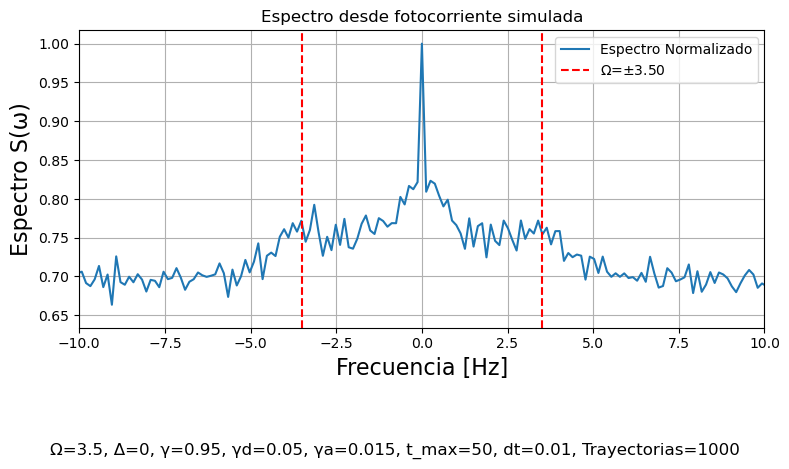
\includegraphics[width=9cm,height=7cm]{fig6_picoangosto.png}
\caption{\label{fig:espectroHeterodino} 
Espectro estacionario simulado por detecci\'on heterodina. 
(a) $\Omega=\gamma_+/4=0.2625 \gamma$, b) $\Omega=3.5 \gamma$. 
$\gamma=1$, $\gamma_d=0.05$, $\gamma_a=0.015$,  $\Delta=0$ }
\end{figure}
%% 
mostrado en la Fig.~\ref{fig:espectroHeterodino}. El decaimiento 
lento se refleja en el pico central angosto sobre el llamado espectro de 
Mollow \cite{Mollow69} del \'atomo de dos niveles.

Un espectro puede medirse anteponiendo un filtro tipo Fabry-Perot al 
detector. En este m\'etodo, sin embargo, la resoluci\'on de estos filtros 
es del orden de MHz, mientras que la resoluci\'on del espectro medido 
por detecci\'on heterodina \cite{BuTa00} es del orden de 1 Hz. Otro caso 
de excelente resoluci\'on, $\sim 0.7$ Hz, de este m\'etodo es el de el 
espectro de resonancia fluorescente de un \'atomo de dos niveles excitado 
muy fuera de resonancia, donde la dispersi\'on es el\'astica, es decir, sin 
mediar absorci\'on \cite{Walther97}.

%%%%%%%%%%%%%%%%%%%%%%%%%%%%%%%%%%%%%
%%%%%%%%%%%%%%%%%%%%%%%%%%%%%%%%%%%%%
\section{Formulaci\'on por Ecuaci\'on Maestra}
La intermitencia en la resonancia fluorescente at\'omica puede 
manifestarse en propiedades de promedio en un ensamble.  Si se realiza el 
promedio de un n\'umero muy grande de trayectorias de $|\Psi_c(t)\rangle$ 
se obtiene el operador de densidad 
$\rho= \overline{ | \Psi \rangle \langle \Psi | }$, que cumple la ecuaci\'on 
maestra (o de Lindblad) 
%
\begin{eqnarray}
\dot{\rho} = -\frac{i}{\hbar} (H_{\mathrm{eff}} \rho -\rho H_{\mathrm{eff}}^{\dag} )
	+\sum_k \mathcal{C}_k \rho \mathcal{C}_k^\dag .
\end{eqnarray}
%%
y describe la din\'amica promedio del sistema. Las trayectorias de saltos 
y las difusivas estudiadas arriba son solo dos de un n\'umero infinito de 
maneras de descomponer la din\'amica promedio, aunque solo unas 
pocas de ellas representan (simulan) experimentos reales. La ecuaci\'on 
anterior puede reescribirse como 
%
\begin{eqnarray}
\dot{\rho} &=& -i [\mathcal{H},\rho] +{\gamma}\mathcal{L}[\sigma_{ge}] \rho 
	+{\gamma_d} \mathcal{L}[\sigma_{ae}] \rho 	
	+ {\gamma_a} \mathcal{L}[\sigma_{ga}] \rho   , 
\end{eqnarray}
%%
donde $\mathcal{H} = \Delta \, \sigma_{eg} \sigma_{ge} 
	+\Omega ( \sigma_{eg} +\sigma_{ge})/2$ 
es el Hamiltoniano \'atomo-l\'aser en la aproximaci\'on de onda rotante, y 
$\mathcal{L}[\mathcal{O}]\rho \equiv \mathcal{O}\rho\mathcal{O}^\dagger 
 - (\mathcal{O}^\dagger\mathcal{O}\rho 
+\rho\mathcal{O}^\dagger\mathcal{O})/2$ 
son superoperadores de decaimiento espont\'aneo. Los operadores 
at\'omicos  $\sigma_{jk} = |j \rangle\langle k|$ obedecen 
$\sigma_{jk} \sigma_{lm} = \sigma_{jm} \delta_{kl}$.  

La tarea ahora es obtener y resolver las ecuaciones para los elementos 
de la matriz, $\rho_{jk} = \langle j| \rho |k\rangle$. Dada la naturaleza 
incoherente del canal de decaimiento $|e \rangle - |a \rangle - |g \rangle$, 
las ecuaciones para las poblaciones $\rho_{jj}$ y las coherencias 
$\rho_{eg}, \rho_{ge}$ se desacoplan de las ecuaciones para las otras 
coherencias. Usando la conservaci\'on de la probabilidad podemos 
eliminar la ecuaci\'on para $\rho_{aa}$. Entonces solo se tiene que 
resolver un sistema de cuatro ecuaciones con cuatro inc\'ognitas que 
escribimos de manera compacta \cite{CaRG16} como 
%
\begin{eqnarray} 	\label{eq:BlochEqs}
\frac{d}{dt}\langle \mathbf{s} (t) \rangle 
	&=& \mathbf{M} \langle \mathbf{s}(t) \rangle +\mathbf{b} 	\,, 
\end{eqnarray}
%%
donde
%
\begin{subequations}
\begin{eqnarray} 	
\mathbf{s} &\equiv&   
	\left( \sigma_{ge},  \sigma_{eg}, \sigma_{ee}, \sigma_{gg}  \right)^T , 
	\qquad  
\mathbf{b} = (0,0,0,\gamma_a)^T 	,  
\end{eqnarray}
%%
%
\begin{eqnarray} 	\label{eq:matrixM}
\mathbf{M} &=& \left( \begin{array}{cccc}
-i \Delta -\gamma_+/2 & 0 & i\Omega/2 & -i\Omega/2 \\ 
0 & i \Delta -\gamma_+/2 & -i\Omega/2 & i\Omega/2 	 \\ 
i\Omega/2 & -i\Omega/2 & - \gamma_+  & 0 		\\ 
-i\Omega/2 & i\Omega/2 & \gamma_- & -\gamma_a 
\end{array}  \right)    \,,
\end{eqnarray}
%%
%
\begin{eqnarray} 
\gamma_+ = \gamma + \gamma_d   , 	\qquad 
\gamma_- = \gamma - \gamma_a . 
\end{eqnarray}
\end{subequations}
%%
%
\begin{figure}[t]
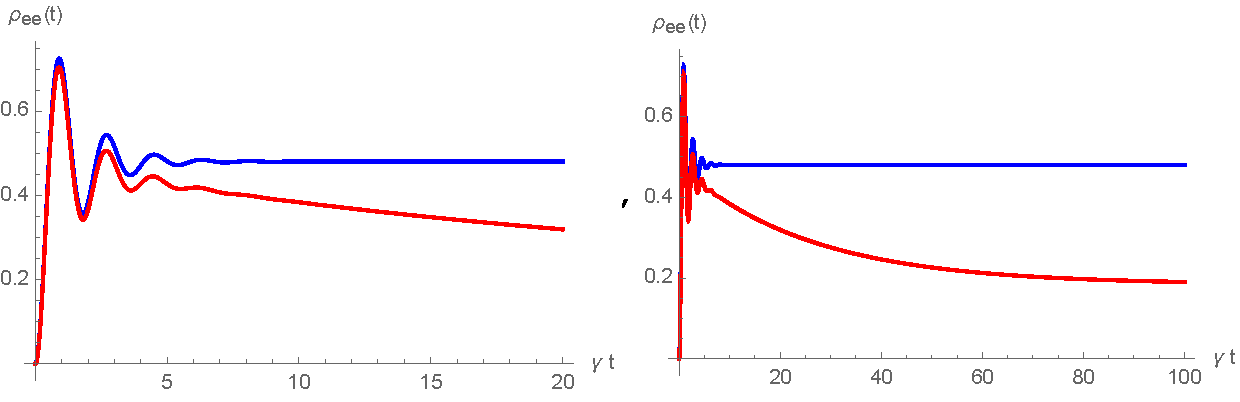
\includegraphics[width=15cm,height=6.0cm]{fig7_epops.pdf} 
\caption{\label{fig:3LA-Pops} Poblaci\'on promedio del estado excitado 
$\rho_{ee}(t)$ con $\Omega = 3.5\gamma$, $\Delta=0$, 
$\gamma_d = 0.05\gamma$, $\gamma_a = 0.015 \gamma$ para un 
\'atomo de dos niveles (azul), y uno de tres niveles (rojo). A la izquierda 
se enfatiza la escala de tiempo corta, $\gamma t_{max} =20$, y a la 
derecha la escala larga, $\gamma t_{max} =100$.  }
\end{figure}
%% 

En general, las ecuaciones se resuelven num\'ericamente. Sin embargo, 
se puede obtener una excelente soluci\'on anal\'itica aproximada en el 
caso en resonancia \'atomo-l\'aser, $\Delta =0$, en el r\'egimen 
$\gamma \gg \gamma_d , \gamma_a$ \cite{CaRG16}. Queremos resaltar 
solamente que la forma de la soluci\'on para la poblaci\'on del estado 
$|e\rangle$, mostrada en la Fig.~\ref{fig:3LA-Pops}, es
%
\begin{equation} 		\label{eq:popE}
\rho_{ee}(t) \sim \rho_{ee}^{ss} +A_+ e^{\lambda_+ t} 
	+A_- e^{\lambda_- t}+B e^{\lambda_2 t}  \,,
\end{equation}
%%
donde $\rho_{ee}^{ss} = \rho_{ee} (t \to \infty)$, $A_{\pm},B$ son 
coeficientes que ignoraremos en nuestra discusi\'on, y 
$\lambda_{\pm,2}$ son los valores propios relevantes que engloban 
la din\'amica del \'atomo: 
%
\begin{subequations}
\begin{eqnarray} 	
\lambda_1 &=& -\gamma_+/2 \,,  \\
%
\lambda_{\pm} &=& -\frac{3\gamma_+}{4} \pm \delta  \,,     \\
%
\lambda_2 &=& -(T_D^{-1} +T_B^{-1})   
	= -\gamma_a \left( 1+ q \frac{\Omega^2 }
	{ 2 \Omega^2 +\gamma^2 +\Delta^2 }  \right) 	\,,  
	\label{eq:small_eigenvalue} \\
	&\ll&  \lambda_1, \lambda_{\pm} \,,  \nonumber 
\end{eqnarray} 
%% 
donde 
%
\begin{eqnarray} 	
\gamma_+ = \gamma +\gamma_d \,,	 	\qquad 
\delta =  \sqrt{(\gamma_+/4)^2 - \Omega^2} \,, \qquad 
q = \frac{\gamma_d}{\gamma_a} \,. 
\end{eqnarray}    
\end{subequations}   
%% 
En la Fig.~\ref{fig:3LA-Pops} se aprecian dos escalas temporales: a 
tiempos cortos, $\gamma t < 10$, ocurre la din\'amica de los per\'iodos 
brillantes, con evoluci\'on coherente amortiguada con eigenvalores 
$\lambda_{\pm}$, muy similar a la del \'atomo de dos niveles, y luego 
ocurre un lento decaimiento al estado estacionario, a raz\'on $\lambda_2$, 
que indica la presencia del estado metaestable en la evoluci\'on. 

Para obtener m\'as informaci\'on del espectro primero reescribimos la 
Ec.(\ref{eq:SpectrumHeterodyne}) como 
%
\begin{eqnarray}
S(\omega) &=& \frac{1}{\pi \rho_{ee}^{st}} \mathrm{Re} 
	\int_0^{\infty} d\tau e^{-i \omega \tau} 
	\langle \sigma_+ (0) \sigma_- (\tau) \rangle_{st}  	\,,
\end{eqnarray}
%%
y luego separamos la din\'amica del dipolo en su valor estacionario 
mas un operador de fluctuaciones, 
$\sigma_{jk} (t) = \langle \sigma_{jk} \rangle_{st} + \Delta \sigma_{jk} (t)$, 
de modo que la autocorrelaci\'on queda escrita como 
%
\begin{eqnarray}
\langle \sigma_+(0) \sigma_-(\tau) \rangle_{st} 
	=\langle \sigma_+ \rangle_{st}  \langle \sigma_- \rangle_{st} 
	+\langle \Delta \sigma_+(0) \Delta \sigma_-(\tau) \rangle_{st}   \,,
\end{eqnarray}
%%
quedando dividido el espectro en dos partes: 
%
\begin{eqnarray}
S(\omega) &=& S_{coh}(\omega) +S_{inc}(\omega) 	\,.
\end{eqnarray}
%%

La parte incoherente (debida a fluctuaciones del dipolo), mostrada en la 
Fig.~\ref{fig:3LA-WK}, es 
%
\begin{eqnarray} 	\label{eq:SincDef}
S_{inc}(\omega) &=& 
\frac{1}{\pi \rho_{ee}^{st}} \mathrm{Re} \int_0^{\infty}  d\tau e^{-i \omega \tau} 
	\langle \Delta \sigma_+(0) \Delta \sigma_-(\tau) \rangle_{st}  	
	\nonumber 	 \\ 
&=& \frac{1}{\pi \rho_{ee}^{st}} \left[ 
	C_+ \frac{ \lambda_+}{\omega^2 +\lambda_+^2}  
	+C_- \frac{ \lambda_-}{\omega^2 +\lambda_-^2}  
	 -C_1 \frac{ \lambda_1}{\omega^2 +\lambda_1^2} 
	-C_2 \frac{ \lambda_2}{\omega^2 +\lambda_2^2}  \right]	\,.
\end{eqnarray}
%%
Los t\'erminos con ($C_1, \lambda_1$) y ($C_{\pm}, \lambda_{\pm}$) 
corresponden a las bandas central y laterales, respectivamente, mientras 
que el t\'ermino con $(C_2,\lambda_2)$ corresponde al pico angosto. 
La anchura del pico angosto esta muy bien aproximada por $-\lambda_2$ 
con valores en el intervalo $(\gamma_a, \gamma_a(1+q/2))$ al 
incrementar la frecuencia de Rabi $\Omega$. 
%
\begin{figure}[h]
\includegraphics[width=9cm,height=8cm]{fig8_IncSpectra.pdf}
\caption{\label{fig:3LA-WK} Espectro estacionario. 
(a) $\Omega=\gamma_+/4=0.2625 \gamma$, b) $\Omega=3.5 \gamma$. 
$\gamma=1$, $\gamma_d=0.05$, $\gamma_a=0.015$,  $\Delta=0$ }
\end{figure}
%% 

La parte coherente, debida al dipolo promedio, es 
%
\begin{eqnarray} 	\label{eq:ScohDef}
S_{coh}(\omega) &=& \frac{|\rho_{eg}^{st}|^2}{\pi \rho_{ee}^{st}} \mathrm{Re} 
	\int_0^{\infty}  e^{-i \omega \tau} d\tau 	
	= \frac{|\rho_{eg}^{st}|^2}{\pi \rho_{ee}^{st}}  \delta(\omega) \nonumber \\
&=& \frac{\gamma_+^2 +4 \Delta^2}
	{\pi \left[ (2+q)\Omega^2 +\gamma_+^2 +4 \Delta^2 \right] } \delta(\omega) 
	= I_{coh}^{A3N} \delta(\omega) \,. 	 
\end{eqnarray}
%% 
Por el factor $q$ en el denominador, se ve que 
$I_{coh}^{A2N} < I_{coh}^{A3N}$. La diferencia se refleja en la intensidad 
del pico angosto:
%
\begin{eqnarray} 	
I_{ep} &=&  I_{coh}^{A2N} - I_{coh}^{A3N} 	\\
&=& \frac{ \Omega^2 \left[ q (\gamma^2 +4 \Delta^2) -2\gamma_d \gamma_+ \right] }
{ \left[ \Omega^2 +\gamma^2 +4 \Delta^2 \right] 
\left[ (2+q)\Omega^2 +\gamma_+^2 +4 \Delta^2 \right] }	\,,  \nonumber
\end{eqnarray}
%%
donde $I_{coh}^{A2N}$ se obtiene haciendo $q=0$ y reemplazando 
$\gamma_+$ por $\gamma$. El pico es m\'aximo cuando  
$\Omega \approx 3\gamma/4$, y peque\~no para campos d\'ebiles 
($I_{ep} \propto \Omega^2$) y muy fuertes ($I_{ep} \propto \Omega^{-2}$). 


%%%%%%%%10%%%%%%%%20%%%%%%%%30%%%%%%%%40%%%
%%%%%%%%%%%%%%%%%%%%%%%%%%%%%% new section
\section{Discusi\'on y Conclusiones}
La intermitencia de la resonancia fluorescente ha sido un tema de gran 
inter\'es desde mediados de los 1980's \cite{PlKn98}. Fue una de las 
razones del uso de ecuaciones estoc\'asticas de Schr\"odinger por el 
estudio de la disipaci\'on de un \'atomo individual, en contraste a la de 
un gas o un s\'olido. Tambi\'en se ha usado con gran provecho en la 
espectroscop\'ia de alta precisi\'on, de particular relevancia en los 
modernos relojes at\'omicos \'opticos.   

En este trabajo presentamos dos contribuciones originales: la distribuci\'on 
de tiempos de retorno, que enfatiza la din\'amica a tiempos largos; y la 
simulaci\'on del espectro por medio de trayectorias cu\'anticas difusivas, 
mejor adaptadas a la realizaci\'on experimental, que las de saltos. 
Tambi\'en se muestran resultados menores que aclaran algunos aspectos 
del problema.    




%%%%%%%%10%%%%%%%%20%%%%%%%%30%%%%%%%%40
%%%%%%%%50%%%%%%%%60%%%%%%%%70%%%
\section{Agradecimientos} 
KMF agradece a SECIHTI por apoyo mediante beca No. CVU: 2056019 


%%%%%%%%%%%%%%%%%%%%%%%  REFERENCES %%%%%%%%
\begin{references} %\begin{thebibliography}
%
\bibitem{Bohr13} N. Bohr, Philos. Mag. \textbf{26}, 476 (1913).   
%
\bibitem{Dehmelt75} H. G. Dehmelt, Bull. Am. Phys. Soc. \textbf{20}, 60 
(1975),
%
\bibitem{NaSD86} W.~Nagourney, J.~Sandberg, and H.~Dehmelt,  
Phys. Rev. Lett. \textbf{56}, 2797 (1986).
%
\bibitem{SNBT86} Th.~Sauter, W.~Neuhauser, R.~Blatt, and P.~E.~Toschek,   
Phys. Rev. Lett. \textbf{57}, 1696 (1986).
%
\bibitem{BHIW86} J.~C.~Bergquist, R.~G.~Hulet, W.~M.~Itano, and 
D.~J.~Wineland, Phys. Rev. Lett. \textbf{57}, 1699 (1986).
%
\bibitem{PlKn98} M.~B. Plenio and P.~L. Knight, Rev. Mod. Phys. 
\textbf{70}, 101 (1998). 
%
\bibitem{BuTa00} V. B\"uhner and Chr. Tamm, Phys. Rev. A 
	\textbf{61}, 061801 (2000). 
%
\bibitem{HePl95} G.~C. Hegerfeldt and M.~B. Plenio, Phys. Rev. A 
\textbf{52}, 3333 (1995). 
%
\bibitem{GaKK95} B.~M. Garraway, M.~S. Kim, and P.~L. Knight, 
	Opt. Commun. \textbf{117}, 560 (1995).
%
\bibitem{EvKe02} J. Evers and Ch. H. Keitel, Phys. Rev. A 
\textbf{65}, 033813 (2002). 
%
\bibitem{CaRG16} H.~M. Castro-Beltr\'an, R. Rom\'an-Ancheyta, and 
L. Guti\'errez, Phys. Rev. A \textbf{93}, 033801 (2016). 
%
\bibitem{PeKn88} D.~T. Pegg and P.~L. Knight, Phys. Rev. A 
\textbf{37}, 4303 (1988);  D.~T. Pegg and P.~L. Knight, J. Phys. D: 
Appl. Phys. \textbf{21}, S128 (1988). 
%
\bibitem{Mollow69} B.~R. Mollow, Phys. Rev. \textbf{188}, 1969 (1969). 
%
\bibitem{Walther97} J. T. H\"offges, H. W. Baldauf, W. Lange, and 
H. Walther, J. Mod. Opt., \textbf{44}, 1999 (1997). 
%
\bibitem{Carm93} H.~J. Carmichael, \textit{Open Systems Approach to 
Quantum Optics} (Springer, Berlin, 1993). 
%
%\bibitem{StHB09} F.~D. Stefani, J.~P. Hoogenboom, and E. Barkai, Phys. 
%Today \textbf{62}(2), 34 (2009). 
%
%\bibitem{LeBa15} N.~Leibovich and E.~Barkai, Phys. Rev. Lett. \textbf{115}, 
%080602 (2015).  
%
 %\bibitem{Minev18} Z.~K.~Minev et al, arXiv 1803.00545v1.
 

\end{references} %\end{thebibliography}


\end{document}			%%% END OF DOCUMENT


